\section{2D 2G Quarter Core}
\subsection{Equations}
This problem is a more traditional $k$-eigenvalue criticality problem using neutron diffusion.  We simulate a benchmark reactor core by imposing reflecting conditions on the left and bottom boundaries of a quarter-core geometry.  The governing PDE for this equation is still
\begin{equation}
-\drv{}{x}D_g\drv{\phi_g}{x}+(\Sigma_{g,a}+\Sigma_{g,s})\phi_g = \sum_{g'}\sigma_{s}^{g'\to g}\phi_{g'} + \frac{\chi_{g}}{k}\sum_{g'}\nu_{g'}\sigma_{f,g'}\phi_{g'},\hspace{15pt} g\in[1,2],
\end{equation}
\begin{equation}
\Sigma_{g,a}=\Sigma_{g,c}+\Sigma_{g,f},
\end{equation}
where $g$ denotes the energy group, $D$ is the group diffusion cross section; $\phi$ is the group flux, $x$ is the location within the problem; $\Sigma_a,\Sigma_s,\Sigma_f$ are the macroscopic absorption, scattering, and fission cross sections respectively; $k$ is the criticality factor eigenvalue and quantity of interest; and $\chi$ is the fraction of neutrons born into an energy group.  In this case, we consider only downscattering, and fission neutrons are only born into the high energy group ($\Sigma_s^{2\to1}=\chi_2=0$).  Our coupled equations are
\begin{equation}
-\drv{}{x}D_1\drv{\phi_1}{x}+(\Sigma_{1,a}+\Sigma_s^{1\to2})\phi_1 = \frac{1}{k}\sum_{g'=1}^2\nu_{g'}\sigma_{f,g'}\phi_{g'},
\end{equation}
\begin{equation}
-\drv{}{x}D_2\drv{\phi_2}{x}+\Sigma_{2,a}\phi_2 = \sigma_{s}^{1'\to 2}\phi_1,
\end{equation}
\begin{equation}
\Sigma_{g,a}=\Sigma_{g,c}+\Sigma_{g,f}.
\end{equation}

\subsection{Materials and Geometry}
The two-dimensional core is shown in Fig. \ref{coremap} and the material properties are listed in Table \ref{tab:coremats}.
\begin{figure}[h]
\centering
   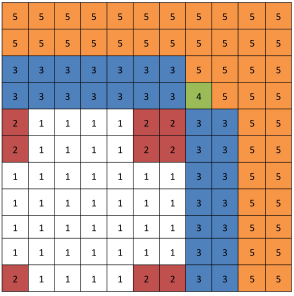
\includegraphics[width=0.4\textwidth]{../graphics/core}
   \caption{Core Map}
   \label{coremap}
\end{figure}
\begin{table}[h]
\centering
\begin{tabular}{c c | c c c c}
Region & Group & $D_g$ & $\Sigma_{c,g}$ & $\nu\Sigma_{f,g}$ & $\Sigma_s^{1,2}$ \\ \hline
1 & 1 & 1.255    & 4.602e-3 & 4.602e-3 & 2.533e-2 \\
  & 2 & 2.11e-1  & 5.540e-2 & 1.091e-1 & \\ \hline
2 & 1 & 1.268    & 4.609e-3 & 4.609e-3 & 2.767e-2 \\
  & 2 & 1.902e-1 & 8.675e-2 & 8.675e-2 & \\ \hline
3 & 1 & 1.259    & 6.083e-3 & 4.663e-3 & 2.617e-2 \\
  & 2 & 2.091e-1 & 4.142e-2 & 1.021e-1 & \\ \hline
4 & 1 & 1.259    & 4.663e-3 & 4.663e-3 & 2.617e-2 \\
  & 2 & 2.091e-1 & 3.131e-2 & 1.021e-1 & \\ \hline
5 & 1 & 1.257    & 6.034e-4  & 0 & 4.754e-2 \\
  & 2 & 1.592e-1 & 1.911e-2  & 0 & 
\end{tabular}
\caption{Basic Material Properties for Core}
\label{tab:coremats}
\end{table}

\subsection{Uncertainty Quantification}
This problem also does not have a convenient general analytic solution.  We can express the solver as
\begin{equation}
U(p;\theta) = k(p;\Sigma_{2,c}),
\end{equation}
where
\begin{equation}
p=(D_g,\Sigma_{1,c},\Sigma_{g,s},\nu_g,\Sigma_{g,f},\chi_g),\hspace{20pt}g\in[1,2].
\end{equation}
While $\phi_g(x)$ might also be considered a parameter, it is an output value solved simultaneously with $k$.

\subsubsection{Uniform Uncertainty}
For this test we consider $\theta=\Sigma_{2,c}$ uniformly distributed as $\theta\in\mathcal{N}(0.0454,0.0654s)$. Tabular data for mean and variance convergence is in Table \ref{tab:2dcrit uni}, and the pdfs obtained are in Fig. \ref{fig:2dcrit uni}.

The PCESC runs all made use of order 32 quadrature to integrate chaos moments.

\begin{table}
\begin{center}
\begin{tabular}{c c|l l}
type & runs/order & mean & variance \\ \hline
MC & $1\times10^6$ & 1.00406413634 & 0.000446173081079 \\
SC & 2  & 1.00416405471 & 0.000375112851817 \\
SC & 4  & 1.00416405471 & 0.000390962150246 \\
SC & 8  & 1.00416405471 & 0.000406864600682 \\
SC & 16 & 1.00416405471 & 0.000421349517322 \\
SC & 32 & 1.00416405471 & 0.000425027572716
\end{tabular}
\end{center}
\caption{Convergence of Mean, Variance for 2D2G Case}
\label{tab:2dcrit uni}
\end{table}

\begin{figure}[h!]
\centering
   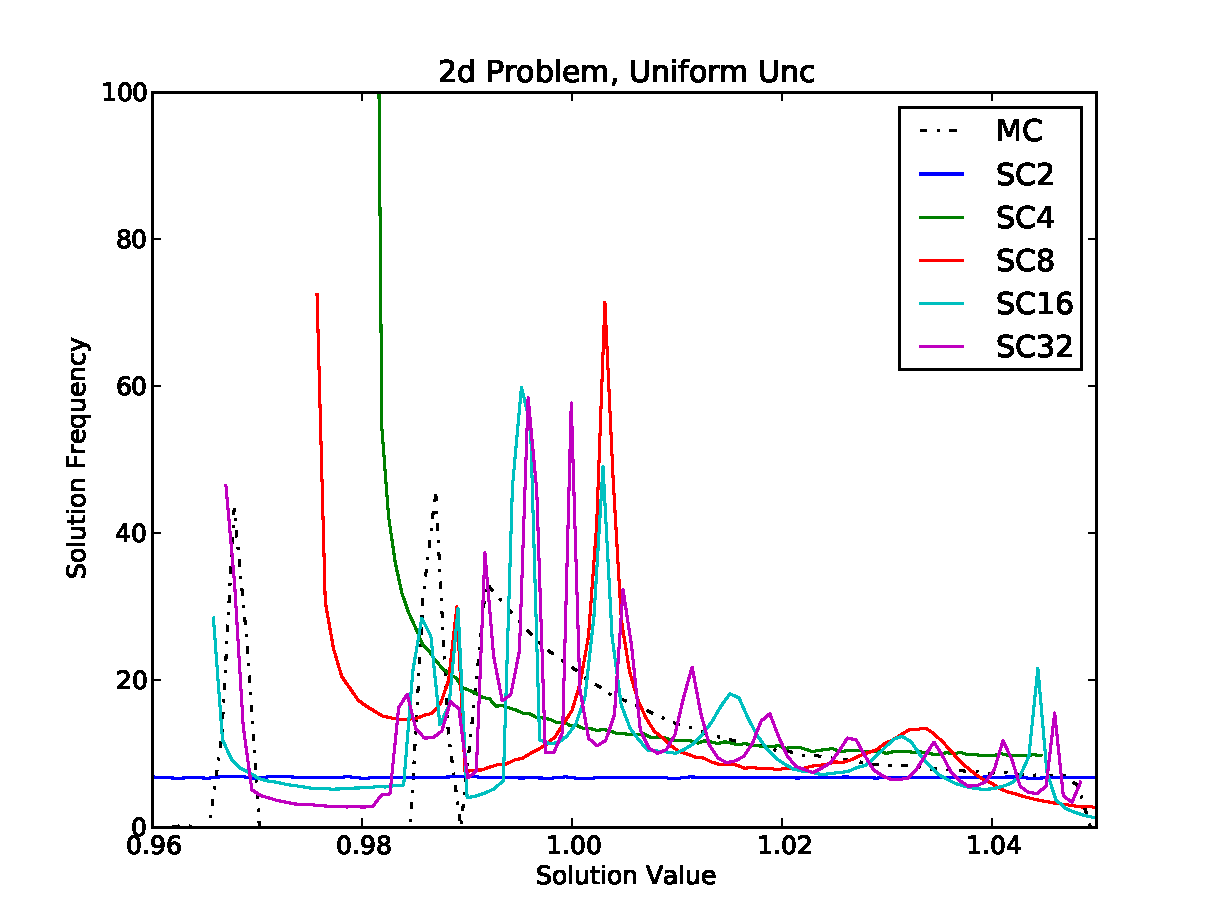
\includegraphics[width=\textwidth]{../graphics/2d_uniform_pdfs}
   \caption{Solution PDF Convergence, 2D2G Case}
   \label{fig:2dcrit uni}
\end{figure}

\subsubsection{Normal Uncertainty}
For this test we consider $\theta=\Sigma_{2,c}$ normally distributed as $\theta\in\mathcal{N}(0.0554,0.01^2)$. Tabular data for mean and variance convergence is in Table \ref{tab:2dcrit}, and the pdfs obtained are in Fig. \ref{fig:2dcrit}.  Once again, it is important to note that the Monte Carlo sampling was restricted to values within 3 standard deviations of the mean; as such, the means and variances obtained directly through Monte Carlo sampling are not representative of the full uncertainty space.  This truncation of the distribution is enforced because without such a restriction, it is possible to sample physically untenable values for $\Sigma_{2,c}$, including negative values.

The PCESC runs all made use of order 32 quadrature to integrate chaos moments.

\begin{table}
\begin{center}
\begin{tabular}{c c|l l}
type & runs/order & mean & variance \\ \hline
MC & $6\times10^5$ & 1.01333702129 & 0.00160652595587 \\
SC & 2  & 1.01643813464 & 0.00138703446968 \\
SC & 4  & 1.01643813464 & 0.00184314998697 \\
SC & 8  & 1.01643813464 & 0.00184690058216 \\
SC & 16 & 1.01643813464 & 0.00184724103523 \\
SC & 32 & 1.01643813464 & 0.00184726152781
\end{tabular}
\end{center}
\caption{Convergence of Mean, Variance for 2D2G Case}
\label{tab:2dcrit}
\end{table}

\begin{figure}[h!]
\centering
   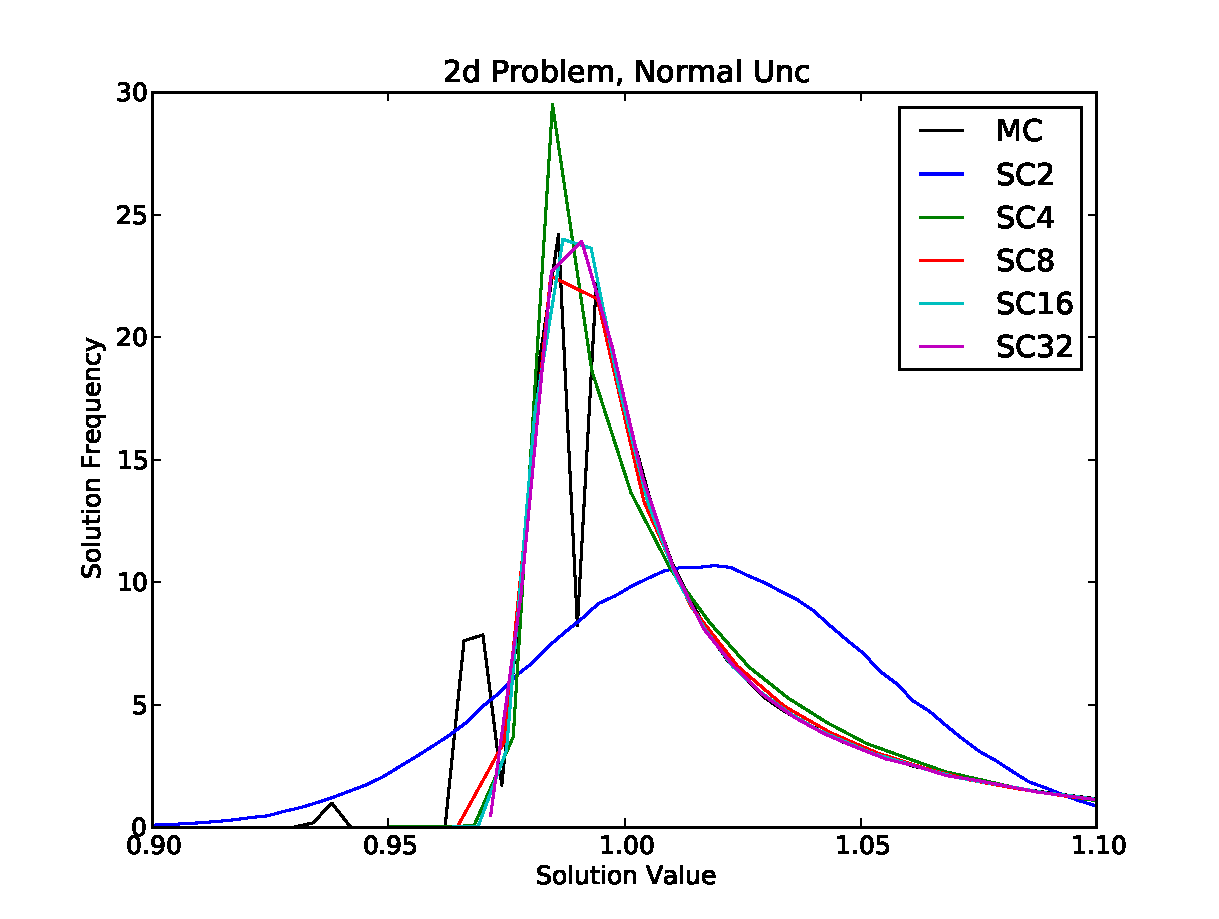
\includegraphics[width=\textwidth]{../graphics/2d_normal_pdfs}
   \caption{Solution PDF Convergence, 2D2G Case}
   \label{fig:2dcrit}
\end{figure}


%
%\begin{figure}[h!]
%\centering
%   \includegraphics[width=\textwidth]{../graphics/}
%   \label{}
%   \caption{}
%\end{figure}
%\begin{table}
%\begin{center}
%\begin{tabular}{c c|l l| r}
%type & runs/order & mean & variance & run time (sec) \\ \hline
%MC & 1\times10^6 &  &  & \\
%SC & 2 & & & \\
%SC & 4 & & & \\
%SC & 8 & & & \\
%SC & 16 & & &
%\end{tabular}
%\end{center}
%\caption{}
%\label{}
%\end{table}
%
%\begin{figure}[h!]
%\centering
%   \includegraphics[width=\textwidth]{../graphics/}
%   \label{}
%   \caption{}
%\end{figure}
